% Copyright 2004 by Till Tantau <tantau@users.sourceforge.net>.
%
% In principle, this file can be redistributed and/or modified under
% the terms of the GNU Public License, version 2.
%
% However, this file is supposed to be a template to be modified
% for your own needs. For this reason, if you use this file as a
% template and not specifically distribute it as part of a another
% package/program, I grant the extra permission to freely copy and
% modify this file as you see fit and even to delete this copyright
% notice. 

\documentclass{beamer}
\usepackage{graphicx}

% There are many different themes available for Beamer. A comprehensive
% list with examples is given here:
% http://deic.uab.es/~iblanes/beamer_gallery/index_by_theme.html
% You can uncomment the themes below if you would like to use a different
% one:
%\usetheme{AnnArbor}
%\usetheme{Antibes}
%\usetheme{Bergen}
%\usetheme{Berkeley}
%\usetheme{Berlin}
%\usetheme{Boadilla}
%\usetheme{boxes}
%\usetheme{CambridgeUS}
%\usetheme{Copenhagen}
%\usetheme{Darmstadt}
%\usetheme{default}
%\usetheme{Frankfurt}
%\usetheme{Goettingen}
%\usetheme{Hannover}
%\usetheme{Ilmenau}
%\usetheme{JuanLesPins}
%\usetheme{Luebeck}
\usetheme{Madrid}
%\usetheme{Malmoe}
%\usetheme{Marburg}
%\usetheme{Montpellier}
%\usetheme{PaloAlto}
%\usetheme{Pittsburgh}
%\usetheme{Rochester}
%\usetheme{Singapore}
%\usetheme{Szeged}
%\usetheme{Warsaw}

\title{High Resolution Sparse Voxel DAGs}


\author{Prateek Chandan \and Anurag Shirolkar}
% - Give the names in the same order as the appear in the paper.
% - Use the \inst{?} command only if the authors have different
%   affiliation.

\institute[IIT Bombay] % (optional, but mostly needed)
{
  \inst{}%
  Department of Computer Science\\
  IIT Bombay
}
% - Use the \inst command only if there are several affiliations.
% - Keep it simple, no one is interested in your street address.

\date{CS 775}
% - Either use conference name or its abbreviation.
% - Not really informative to the audience, more for people (including
%   yourself) who are reading the slides online

\subject{Advanced Computer Graphics}
% This is only inserted into the PDF information catalog. Can be left
% out. 

% If you have a file called "university-logo-filename.xxx", where xxx
% is a graphic format that can be processed by latex or pdflatex,
% resp., then you can add a logo as follows:

% \pgfdeclareimage[height=0.5cm]{university-logo}{university-logo-filename}
% \logo{\pgfuseimage{university-logo}}

% Delete this, if you do not want the table of contents to pop up at
% the beginning of each subsection:
\AtBeginSubsection[]
{
  \begin{frame}<beamer>{Outline}
    \tableofcontents[currentsection,currentsubsection]
  \end{frame}
}

% Let's get started
\begin{document}

\begin{frame}
  \titlepage
\end{frame}

\begin{frame}{Outline}
  \tableofcontents
  % You might wish to add the option [pausesections]
\end{frame}

% Section and subsections will appear in the presentation overview
% and table of contents.
\section{Abstract}

	\begin{frame}{Abstract}
	\begin{itemize}
		\item {
		A binary voxel grid can be represented more efficiently by using a Directed Acyclic Graph(DAG) than Sparse Voxel Octree(SVO)
		}
		\item {
			Along with efficient encoding of empty regions , DAG allows efficient encoding of identical regions as nodes are allowed to share pointers
		}
		\item {
			This paper presents a bottom-up algorithm to reduce a SVO to DAG
		}
		\item {
			The memory consumption of DAG is significantly smaller and it would fit in memory where SVO won't
		}
		\item {
			DAG requires no decompression and can be traversed easily
		}
		\item {
			This paper demonstrates this by ray tracing hard and soft shadows , ambient occlusion , and primary rays in extremly high resolution DAG at speed at par or even faster than voxel and triangle GPU ray tracing.
		}
	\end{itemize}
\end{frame}

\section{Introduction}

% You can reveal the parts of a slide one at a time
% with the \pause command:
\begin{frame}{Introduction}
  \begin{itemize}
  \item {
    There is increased interest in evaluating secondary rays for effects as reflection, shadows and indirect illumination. Due to the incoherence, a scondary scene representation is required with strict memory budget
    
  }
  \item {   
    This acceleration structure has to be resident on RAM for effiecient access.
  }
  \item{
  However this is problematic when triangle meshes are augmented with displacement maps as they become infeasibly large to millions of polygons
  \pause
  }
  \item {
  	Recently Sparse Voxel Octree(SVO) has been used as a secondary scene representation, since they provide implicit LOD mechanism and can be efficiently ray traced in real time.
  }
  \item {
  	At high resolution, SVO is still too much memory expensive, therefore it's application has been limited }
  \end{itemize}
\end{frame}

\begin{frame}{Introduction}
  \begin{itemize}
  \item {
  		The data structure \textbf{DAG} allows for extremly high resolution enabling us to improve image quality, decrease discretization artifacts, explore high frequency effects like sharp shadows in large scenes.
    }
 
  \end{itemize}
  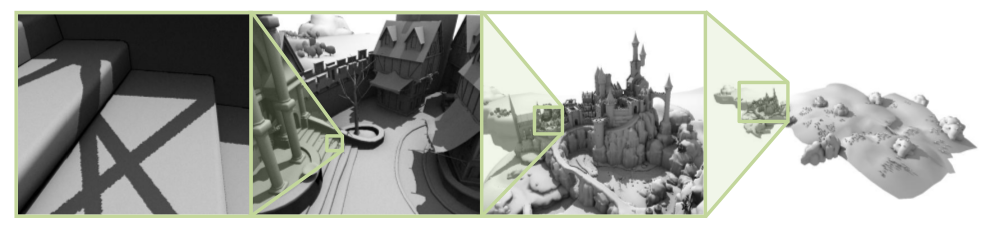
\includegraphics[scale=0.36]{fig1}{C Figure 1: The EPIC CITADEL scene voxelized to a $128K^3$ resolution and stored as a Sparse Voxel DAG.}
\end{frame}

\begin{frame}{Introduction}
  \begin{itemize}
  \item {
  		The paper presents and efficient technique for reducing the size of SVO by merging common subtrees and transforming to a DAG.
    }
    \item{
    	This can dramatically reduce memory demands in real world scenes and scales even better with increased resolutions.
    }
    \item{
    	This is based on assumption that the original DAG contains a large amount of redundant subtrees
    }
    \item{
    	This paper implements and evaluates algorithms for calculating hard and soft shadows and ambitent occlusion by Ray tracing in DAG 
    }
 
  \end{itemize}
 
\end{frame}

\section{Previous Work}
\subsection{Sparse Voxel Octrees}
\begin{frame}{Sparse Voxel Octrees}
\end{frame}

\subsection{Common subtree merging}
\begin{frame}{Common subtree merging}
\end{frame}

\subsection{Shadows}
\begin{frame}{Shadows}
\end{frame}

\subsection{Ambient Occlusion}
\begin{frame}{Ambient Occlusion}
\end{frame}

\section{Reducing a Sparse Voxel Tree to a DAG}
\begin{frame}{Reducing a Sparse Voxel Tree to a DAG}
	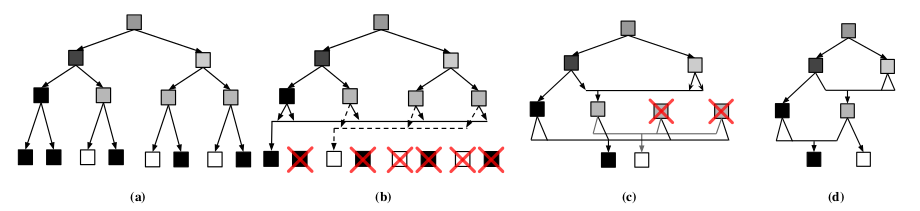
\includegraphics[scale=0.37]{fig2}{ Figure 2:Reducing a sparse voxel tree, illustrated using a binary tree, instead of an octree, for clarity.}
	\begin{enumerate}[a.]
		\item{The original tree.}
		\item{Non-unique leaves are reduced.}
		\item{Now, there are non-unique nodes in the level above the leaves. These are reduced, creating non-unique nodes in the level above this.}
		\item{The process proceeds until we obtain our final directed acyclic graph.}
	\end{enumerate}
\end{frame}

\begin{frame}{Terminology}
	\begin{itemize}
		\item{
		Consider an $N^3$ voxel grid as a scene representation where each cell can be represented by a bit : \textbf{0} if empty and \textbf{1} if it contains geometry
		}
		\item{
			A sparse voxel octree recursivley divided $L$ time gives us a hierarchical representation of and $N^3$ voxel grid, where $N = 2^L$ and L is called as \textit{max level}.
		}
		\item{
			The sparse represnetation is achieved is achieved by culling away nodes that corresponds to empty space
		}
		\item{
			A node is implemented with a \textit{childmask}, a bitmask of 8 bits where bit $i$ tells us if bit $i$  contains a geometry, and a pointer to first of non-empty children.
		}
		\item{
			Child nodes are stored consecutively in memory	
		}
		\item{
			The unique traversal \textit{path}, from root to a specific node in SVO, defines the voxel without storing spatial information explicitly in the node 
		}
	\end{itemize}
\end{frame}


\begin{frame}{The sparse voxel DAG}
	\begin{itemize}
		\item{
		Consider an $N^3$ voxel grid as a scene representation where each cell can be represented by a bit : \textbf{0} if empty and \textbf{1} if it contains geometry
		}
		
	\end{itemize}
\end{frame}

\section{Ray Tracing a Sparse Voxel DAG}

\section{Evaluation}
\subsection{Reduction Speed}
\subsection{Memory Consumption}
\subsection{Traversal Speed}

\section{Conclusion}
\section{Future Work}

\begin{frame}{Blocks}
\begin{block}{Block Title}
You can also highlight sections of your presentation in a block, with it's own title
\end{block}
\begin{theorem}
There are separate environments for theorems, examples, definitions and proofs.
\end{theorem}
\begin{example}
Here is an example of an example block.
\end{example}
\end{frame}

% Placing a * after \section means it will not show in the
% outline or table of contents.
\section*{Summary}

\begin{frame}{Summary}
  \begin{itemize}
  \item
    The \alert{first main message} of your talk in one or two lines.
  \item
    The \alert{second main message} of your talk in one or two lines.
  \item
    Perhaps a \alert{third message}, but not more than that.
  \end{itemize}
  
  \begin{itemize}
  \item
    Outlook
    \begin{itemize}
    \item
      Something you haven't solved.
    \item
      Something else you haven't solved.
    \end{itemize}
  \end{itemize}
\end{frame}



% All of the following is optional and typically not needed. 
\appendix
\section<presentation>*{\appendixname}
\subsection<presentation>*{For Further Reading}

\begin{frame}[allowframebreaks]
  \frametitle<presentation>{For Further Reading}
    
  \begin{thebibliography}{10}
    
  \beamertemplatebookbibitems
  % Start with overview books.

  \bibitem{Author1990}
    A.~Author.
    \newblock {\em Handbook of Everything}.
    \newblock Some Press, 1990.
 
    
  \beamertemplatearticlebibitems
  % Followed by interesting articles. Keep the list short. 

  \bibitem{Someone2000}
    S.~Someone.
    \newblock On this and that.
    \newblock {\em Journal of This and That}, 2(1):50--100,
    2000.
  \end{thebibliography}
\end{frame}

\end{document}


